% Model_LocalCartesian.tex
% Face-on view of the source plane, showing the local CARTESIAN coordinate
% system (beta-tilde_1, beta-tilde_2) centred on the source, together with
% the global coordinate directions (beta_1, beta_2).
% Companion figure to Model_LocalPolar.tex (lens plane / polar coordinates).
% Colour palette chosen at mid luminance so it stays legible on both
% white and black page backgrounds.
\documentclass[border=4pt]{standalone}
\usepackage{tikz}
\usepackage{amsmath}
\usetikzlibrary{arrows.meta, decorations.markings, calc}

\definecolor{inkcol}{RGB}{125,132,140}
\definecolor{planecol}{RGB}{155,155,155}
\definecolor{imgcol}{RGB}{205,165,45}
\definecolor{anglecol}{RGB}{170,95,200}

% the kidney/banana shaped blob used for the source, shifted so that the
% pic's local origin (0,0) -- where the local coordinate system below is
% centred -- falls inside the filled shape, roughly at its "light centre".
\tikzset{
  kidney/.pic={
    \fill[imgcol]
      (-0.6,1) .. controls (-0.05,0.95) and (0.4,0.4)  .. (0.4,0)
               .. controls (0.4,-0.4)  and (-0.05,-0.95) .. (-0.6,-1)
               .. controls (-0.45,-0.75) and (-0.25,-0.3) .. (-0.25,0)
               .. controls (-0.25,0.3)  and (-0.45,0.75) .. cycle;
  }
}

\begin{document}
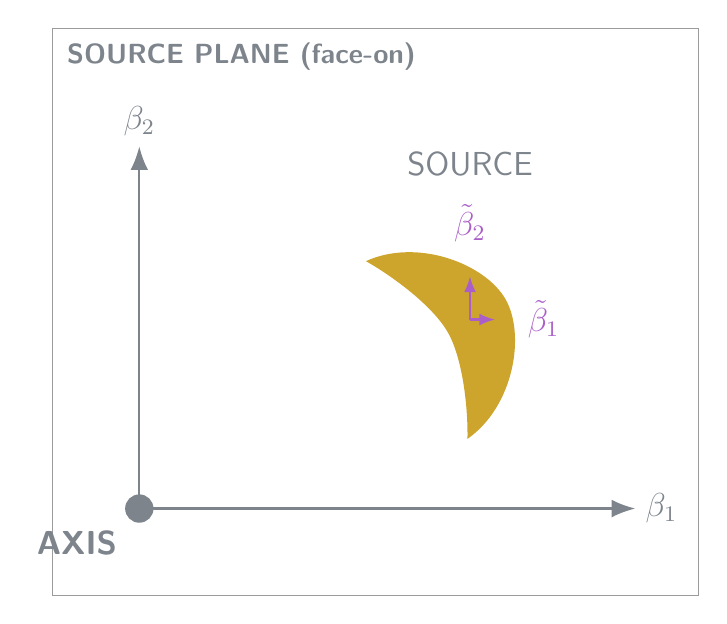
\begin{tikzpicture}[
    >=Latex,
    line width=1pt,
    font=\sffamily
  ]

  % --- coordinates -------------------------------------------------------
  \coordinate (Origin) at (0,0);
  \coordinate (SrcPos) at (4.2,2.4);

  % --- frame, representing the source plane viewed face-on ---------------
  \draw[planecol, thin] (-1.1,-1.1) rectangle (7.1,6.1);
  \node[inkcol, font=\sffamily\bfseries, anchor=north west] at (-1.05,6.05) {SOURCE PLANE (face-on)};

  % --- global coordinate axes, centred on the optical axis ----------------
  \draw[inkcol, thick, -{Latex[length=3mm]}] (Origin) -- (6.3,0) node[right, font=\sffamily\large] {$\beta_1$};
  \draw[inkcol, thick, -{Latex[length=3mm]}] (Origin) -- (0,4.6) node[above, font=\sffamily\large] {$\beta_2$};
  \fill[inkcol] (Origin) circle (0.18);
  \node[inkcol, font=\sffamily\bfseries\large, anchor=north east] at (-0.15,-0.15) {AXIS};

  % --- the source itself (kidney/banana shape) ----------------------------
  \pic[scale=1.3, rotate=29.74] at (SrcPos) {kidney};
  \node[inkcol, font=\sffamily\large, anchor=south] at ($(SrcPos)+(0,1.7)$) {SOURCE};

  % --- local Cartesian axes (beta-tilde_1, beta-tilde_2), parallel to the
  % global axes, centred on the source's "light centre"; both tips land
  % inside the source itself ------------------------------------------------
  \draw[anglecol, thick, -{Latex[length=2mm]}]
    (SrcPos) -- ($(SrcPos)+(0.32,0)$);
  \node[anglecol, font=\sffamily\large, anchor=west] at ($(SrcPos)+(0.6,0)$) {$\tilde{\beta}_1$};

  \draw[anglecol, thick, -{Latex[length=2mm]}]
    (SrcPos) -- ($(SrcPos)+(0,0.55)$);
  \node[anglecol, font=\sffamily\large, anchor=south] at ($(SrcPos)+(0,0.85)$) {$\tilde{\beta}_2$};

\end{tikzpicture}
\end{document}
